\chapter{开源工具}
本章主要介绍一些数学优化、机器学习、搜索引擎等各领域相关的开源工具,对于一些经典的算法框架或实现,如果没有相应的开源工具可供选择,我们会选择收录商业机构的产品。
\section{Apache Lucene}
\section{Xapian}
\href{http://xapian.org/}{Xapian}是一个开源的搜索引擎库,使用C++编写,已经实现多种语言(如Java,Python等)接口。用户可以轻松地为应用添加索引和检索功能,并支持概率信息检索模型和丰富的布尔查询运算。此外,它还是首个支持排序学习(L2R)功能的项目,了解其排序学习框架,可以参考
\href{http://trac.xapian.org/wiki/GSoC2011/LTR/LTRFramework}{GSoC2011}。

\section{Apache Nutch}

\section{Hadoop}
Hadoop是一个分布式系统基础架构,由Apache基金会开发。用户可以在不了解分布式底层细节的情况下,开发出分布式程序,充分利用集群的威力进行高速运算和存储。Hadoop实现了一个分布式文件系统——HDFS。它具有高容错性,设计用来部署在低廉的硬件上,还能提供高传输率以访问应用程序的数据,特别适合于包含超大数据集的应用程序。
\begin{figure}[htbp]
  \centering
  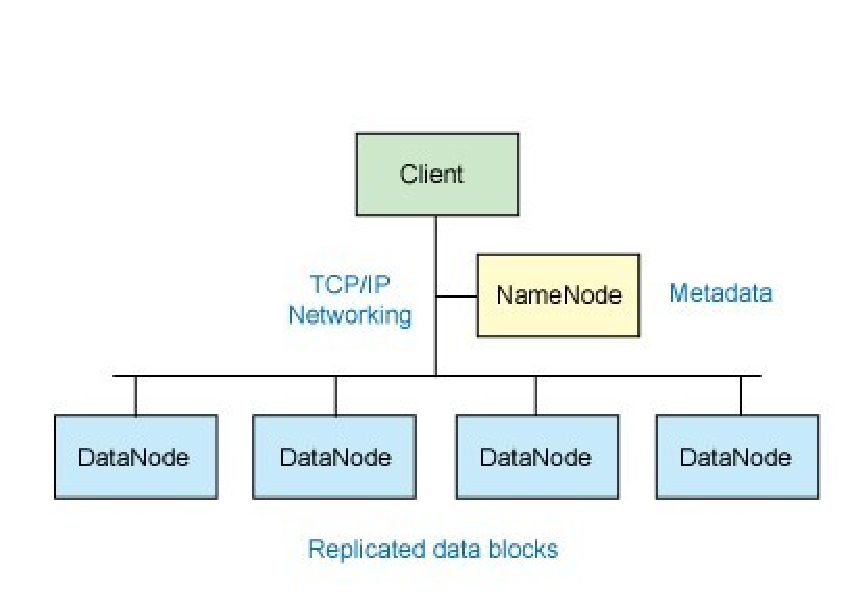
\includegraphics[width=0.65\textwidth]{figures/Hadoop.eps}
  \caption{Hadoop基本架构}\label{fig:hadoop}
\end{figure}

Hadoop的基本架构如图~\ref{fig:hadoop}所示。Hadoop的最底层是HDFS,存储集群中所有存储节点上的文件。HDFS的上一层是MapReduce引擎,由JobTrackers和TaskTrackers组成。一个hadoop集群通常有几十台甚至成百上千台低廉的计算机组成,我们运行的每一个任务都要在这些计算机上做任务的分发,执行中间数据排序及最后结果的汇总,另外还包含节点发现,任务的重试,故障节点替换等维护工作及异常处理,因此说Hadoop就是一个计算模型,是一个分布式的计算模型。

\subsection{MapReduce}
MapReduce是Google公司研究人员提出提出的一种数据处理模型,属于一种函数式编程模式。Google爬虫采集了海量的互联网网页数据,无论是网页解析还是建立索引都是一项艰巨的任务,需要借助成千上万台机器协同完成(也就是分布式并行处理)。为此,研究人员发明了MapReduce数据处理模型~\cite{dean2008mapreduce}。后来,Doug Cutting据此实现了MapReduce 框架,在大量开源人员的共同努力下逐步完善,产生了现今的Hadoop。

MapReduce处理数据主要分成两个阶段:Map阶段和Reduce阶段。Map阶段首先执行,随后进入Reduce阶段。

\section{HtmlParser}

\section{HtmlUnit}
\href{http://sourceforge.net/projects/htmlunit/}{HtmlUnit}是Junit 的扩展测试框架之一,该框架模拟浏览器的行为,开发者可以使用其提供的API对页面的元素进行操作,套用官方网站的话HtmlUnit“是Java程序的浏览器”。HtmlUnit支持HTTP,HTTPS,COOKIE,表单的POST和GET方法,能够对HTML文档进行包装,页面的各种元素都可以被当作对象进行调用,另外对JavaScript的支持也比较好。要正确运行js代码,得能模拟出浏览器环境,包括window对象,document对象等等

\section{Laboratory for Web Algorithmics: LAW}
Research at \href{http://law.di.unimi.it/}{LAW} concerns all algorithmic aspects of the study of the web and of social networks. They are:
\begin{itemize}
\item \textbf{UbiCrawler}: High-performance web crawling
\item \textbf{WebGraph}: Compression of web graphs and social networks
\item \textbf{HyperANF and MG4J}: Analysis of web graphs and social networks. HyperANF was used to compute for the first time second-order statistics about the distance distribution of a large number of web and social graphs
\end{itemize}

\subsubsection{MG4J}
\href{http://mg4j.dsi.unimi.it/}{Manage Gigabytes for Java}(MG4J) is a free full-text search engine for large document collections written in Java. It is a highly customisable, high-performance, full-fledged search engine providing state-of-the-art features (such as BM25/BM25F scoring) and new research algorithms. The big version is a fork of the original MG4J that can handle more than $2^{31}$ terms and documents.

The starting point for understanding MG4J is a look at the \href{http://mg4j.dsi.unimi.it/man/manual/index.html}{tutorial}, which explains how to index a sample collection and query the newly constructed index from the command line or using a browser.

\subsubsection{WebGraph}
\href{http://webgraph.di.unimi.it/}{WebGraph} is a framework to study the web graph. It provides simple ways to manage very large graphs, new compression techniques, Java code and \href{http://law.di.unimi.it/datasets.php}{data sets}. With WebGraph, you can access and analyse very large web graphs and study the phenomena such as PageRank, distribution of graph properties of the web graph, etc.

\section{SeerSuit}
SeerSuite is an application toolkit for digital libraries and search engines; i.e., \href{http://sourceforge.net/projects/citeseerx/}CiteSeer$^X$}, it's developed on Java。

\section{Mahout}
Mahout是Apache Software Foundation(ASF)旗下的一个开源项目,提供一些可扩展的机器学习经典算法的实现,旨在帮助开发人员便捷地创建智能应用程序。它是一个分布式机器学习算法的集合,许多算法(如分类、聚类、协同过滤等)的实现是按照MapReduce的方式实现,可以在Hadoop上运行,并行处理大规模数据。在推荐方面,它实现了一个个性化推荐引擎Taste,其结构如图\ref{fig:taste}所示。

\begin{table}[ht]\caption{Mahout机器学习算法}
\centering
    \begin{tabular}{l|l|l}
        \hline\hline
        类别 & 英文名称 & 中文名称\\
        \hline
        & Logistic Regression & 逻辑回归\\[0.5ex]
        & Bayesian & 贝叶斯\\[0.5ex]
        & SVM & 支持向量机\\[0.5ex]
        分类算法 & Perceptron & 感知器\\[0.5ex]
        & Neural Network & 神经网络\\[0.5ex]
        & Random Forests & 随机森林\\[0.5ex]
        & Restricted Boltzmann Machines & 受限波尔兹曼机\\[1ex]
        \hline
        & Canopy Clustering & Canopy聚类\\[0.5ex]
        & K-means Clustering & K均值算法\\[0.5ex]
        & Fuzzy K-means & 模糊K均值\\[0.5ex]
        & Expectation Maximization & EM聚类\\[0.5ex]
        聚类算法 & Mean Shift Clustering & 均值漂移聚类\\[0.5ex]
        & Hierarchical Clustering & 层次聚类\\[0.5ex]
        & Dirichlet Process Clustering & 狄里克雷过程聚类\\[0.5ex]
        & Latent Dirichlet Allocation & LDA聚类\\[0.5ex]
        & Spectral Clustering & 谱聚类\\[1ex]
        \hline
        回归模型 & Locally Weighted Linear Regression & 局部加权线性回归\\[1ex]
        \hline
        & Non-distributed recommenders & Taste(UserCF, ItemCF, SlopeOne)\\[0.5ex]
        \raisebox{1ex}{推荐算法} & Distributed Recommenders & ItemCF\\[1ex]
        \hline
        & Singular Value Decomposition & 奇异值分解\\[0.5ex]
        & Principal Components Analysis & 主成分分析\\[0.5ex]
        \raisebox{1ex}{维数约减} & Independent Component Analysis & 独立成分分析\\[0.5ex]
        & Gaussian Discriminative Analysis & 高斯判别分析\\[1ex]
        \hline
        关联规则挖掘 & Parallel FP Growth Algorithm & 并行FP Growth算法\\[1ex]
        \hline
        进化算法 & 并行化Watchmaker框架 &\\[1ex]
        \hline
        & RowSimilarityJob & 计算列间相似度\\[0.5ex]
        \raisebox{1ex}{向量相似度计算} & VectorDistanceJob & 计算向量间距离\\[1ex]
        \hline
        非MapReduce算法 & Hidden Markov Models & 隐马尔科夫模型\\[0.5ex]
        \hline
    \end{tabular}\label{tbl:mahout}
\end{table}
\begin{figure}[ht]
  \centering
  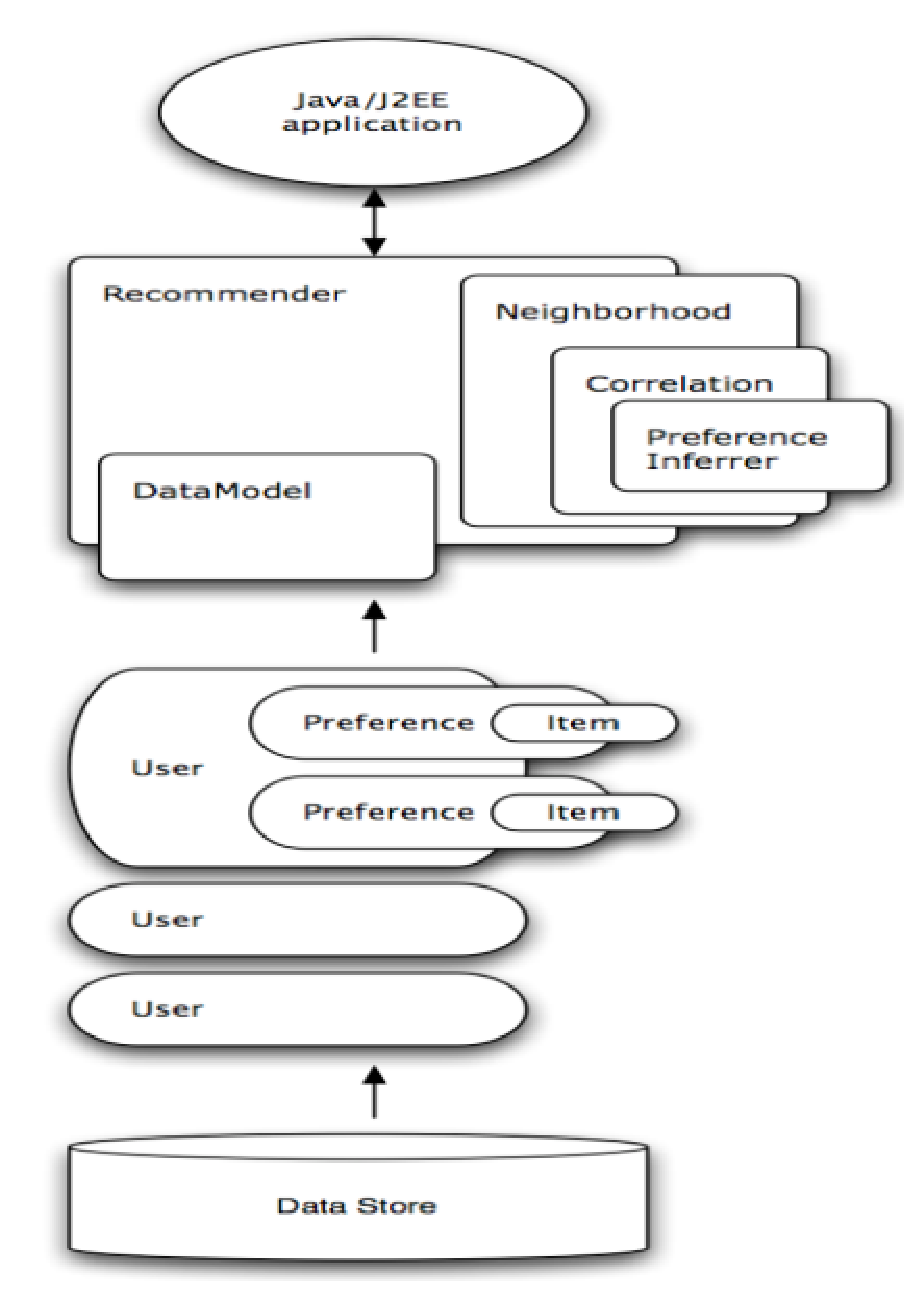
\includegraphics[width=0.6\textwidth,height=11cm]{figures/taste.eps}
  \caption{Mahout Taste}\label{fig:taste}
\end{figure}

\section{PREA}
PREA(Personalized Recommendation Algorithms)工具包\footnote{See \url{http://prea.gatech.edu/index.html}} 实现推荐算法主要是基于矩阵分解(Matrix Factorization)。

\section{SVDFeature}
它是一种矩阵分解的推荐框架\footnote{See \url{http://svdfeature.apexlab.org/}},可以方便的实现SVD、SVD++等单模型性能最高的方法。它使用C++语言开发、代码精炼,可以利用较少的内存实现较大规模的单机版矩阵分解运算。此外,它还含有逻辑回归的实现,方便用来做模型集成。

\section{GraphLab}
它是基于C++开发的一个高性能分布式图挖掘系统\footnote{See \url{http://graphlab.org/}},处理迭代并行计算的能力很强。用它进行海量数据上的随机游走或基于图的推荐算法非常有效。

\section{Lenskit}
由美国明尼苏达大学GroupLens团队开发,系统使用Java语言开发。

\section{LibFM}
第一个项目是矩阵分解的利器\footnote{See \url{http://www.libfm.org/}},实现了马尔科夫链蒙特卡洛优化算法(Markov Chain Monte Carlo,MCMC),要比常见的随机梯度下降法(Stochastic Gradient Descend,SGD)精度更高。第二个同名项目\footnote{See \url{http://www.csie.ntu.edu.tw/\~cjlin/libmf/}}是由LibSVM的作者实现,在矩阵分解并行化方面作出很大贡献。

\section{数学优化}
\begin{table}[htbp]
\centering
\begin{tabular}{|l|c|c|l|}
  \hline
  名称 & 语言 & 支持命令行 & 求解范围\\
  \hline
  \href{http://sourceforge.net/projects/lipside/}{LiPS} & C++ & \XSolid & Linear, integer and goal programming\\
  \href{http://sourceforge.net/projects/lpsolve/}{lp\_solve} & C & \Checkmark & Mixed Integer Linear Programming (MILP)\\
  \href{http://sourceforge.net/projects/javailp/}{Java ILP} & Java & \Checkmark &Interface to solvers such as lp\_solve, Glpk, Mosek, et al.\\
  \href{http://sourceforge.net/projects/glpk-java/}{GLPK} & Java & \Checkmark &Linear and mixed integer mathematical programming\\
  \href{http://www.optaplanner.org/}{OptaPlanner} & Java & \Checkmark &Planning problem,Supports Cloud Computing\\
  \href{http://www.coin-or.org/Clp/userguide/clpuserguide.html}{COIN Linear Program} & C++ & \Checkmark &Linear Programming\\
  \href{http://math.nist.gov/javanumerics/jama/}{JAMA} & Java & \Checkmark &A Java Matrix Package\\
  \hline
\end{tabular}
\end{table}